\part{Architecture}
\section{Rôle des tiers}
\subsection{Front-end}
Le \textit{front-end} va gérer tout ce qui est lié à l'affichage des pages : affichage conditionnel, affichage des résultats, formatage des données\dots L'architecture est la suivante :
\begin{itemize}
	\item \textit{/src/assets} : fichiers statiques (images...)
	\item \textit{/src/components} : fichiers \textbf{.vue} où se trouve des parties de page. Tous à l'exception de \ul{Header.vue} et \ul{Footer.vue} sont appelés dans une des pages définies dans \textit{/src/views}
	\item \textit{/src/config} : fichier de configuration qui regroupe divers paramètres. Actuellement il ne comporte que les \textit{end-points} de l'API
	\item \textit{/src/services} : ficher faisant le lien entre les actions de connexion, inscription et modification des données d'un utilisateur du front et le back
	\item \textit{/src/store} : fichier permettant de manipuler le stockage local de vue (\href{https://vuex.vuejs.org/}{Vuex})
	\item \textit{/src/views} : fichiers \textbf{.vue} regroupant plusieurs components (situés dans \textit{/src/components}) pour afficher le contenu principal de la page
	\item \textit{/src/App.vue} : fichier principal représentant la page
	\item \textit{/src/main.js} : fichier permettant de créer l'application \href{https://vuejs.org/}{VueJs}
\end{itemize}
\subsection{Back-end}
Le \textit{back-end} va lui, récupérer les informations que lui aura envoyé le \textit{front-end} et, en fonction des validations d'identité, renverra les données demandées. L'architecture est la suivante :
\begin{itemize}
	\item \textit{/config} : fichier de configuration. Actuellement il ne comporte que l'URL depuis laquelle il accepte les requêtes
	\item \textit{/middleware} : fichiers contenant les diverses fonctions intermédiaires à exécuter lors des requêtes
	\item \textit{/routes} : contient les fichiers avec toutes les routes et les actions à faire en fonction de la requête et de la ressource demandée. Les routes et actions sont rangées par ressource.
	\item \textit{/services} : fichiers d'aides. Ne contient actuellement qu'une méthode de vérification des json web token.
	\item \textit{/index.js} : creation de l'application \href{https://nodejs.org/en/}{Node.js}
	\item \textit{/db.js} : connexion à la base de données (utilise regex et variables d'environnement)
\end{itemize}
\subsection{Base de données PostgreSQL}
Effectuera les requêtes demandées
\section{Architecture de déploiement}
\subsection{Diagramme}
\begin{figure}[h]
	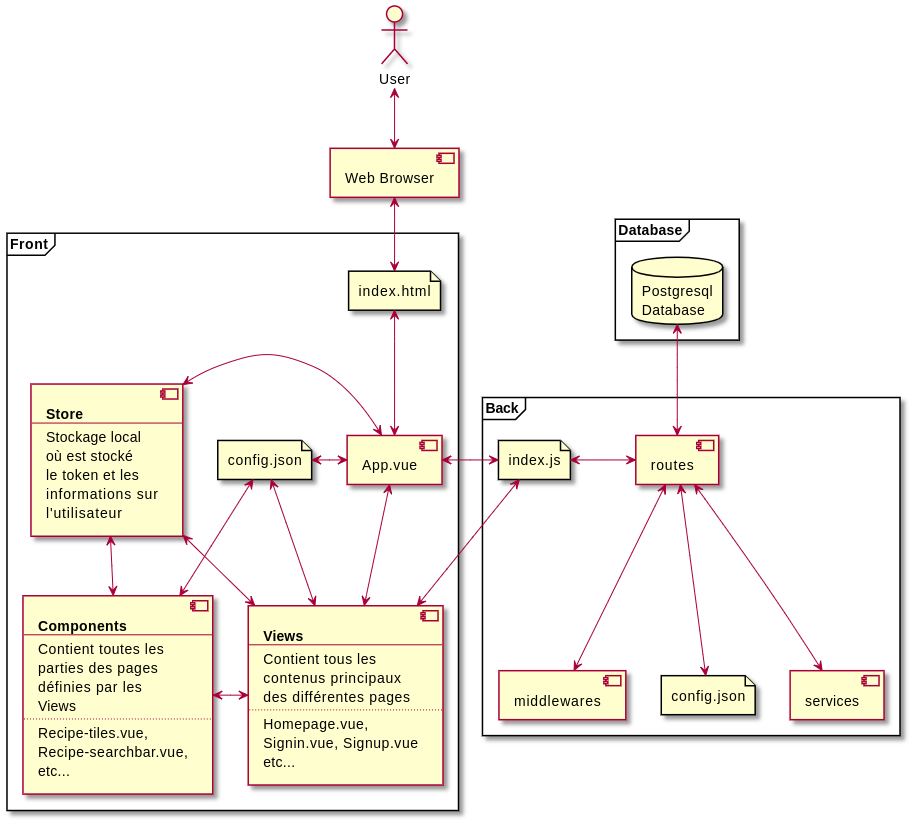
\includegraphics[width=0.9\linewidth]{deploymentArchitecture.png}
	\caption{Architecture du projet}
\end{figure}
\subsection{Déploiement}
La plateforme de déploiement est \href{https://dokku.com/}{Dokku}, un PaaS relativement léger. Le déploiement a été fait sur 2 applications distinctes :
\begin{itemize}
	\item \href{https://polycookerapi.cluster-ig3.igpolytech.fr/}{polycookerapi} : API de PolyCooker
	\item \href{https://polycooker.cluster-ig3.igpolytech.fr/api}{polycooker-cli} : \textit{Front-end} de PolyCooker
\end{itemize}
\pagebreak
\section{Flux d'information}
\begin{figure}[h]
	\centering
	\begin{subfigure}{\linewidth}
		\centering
		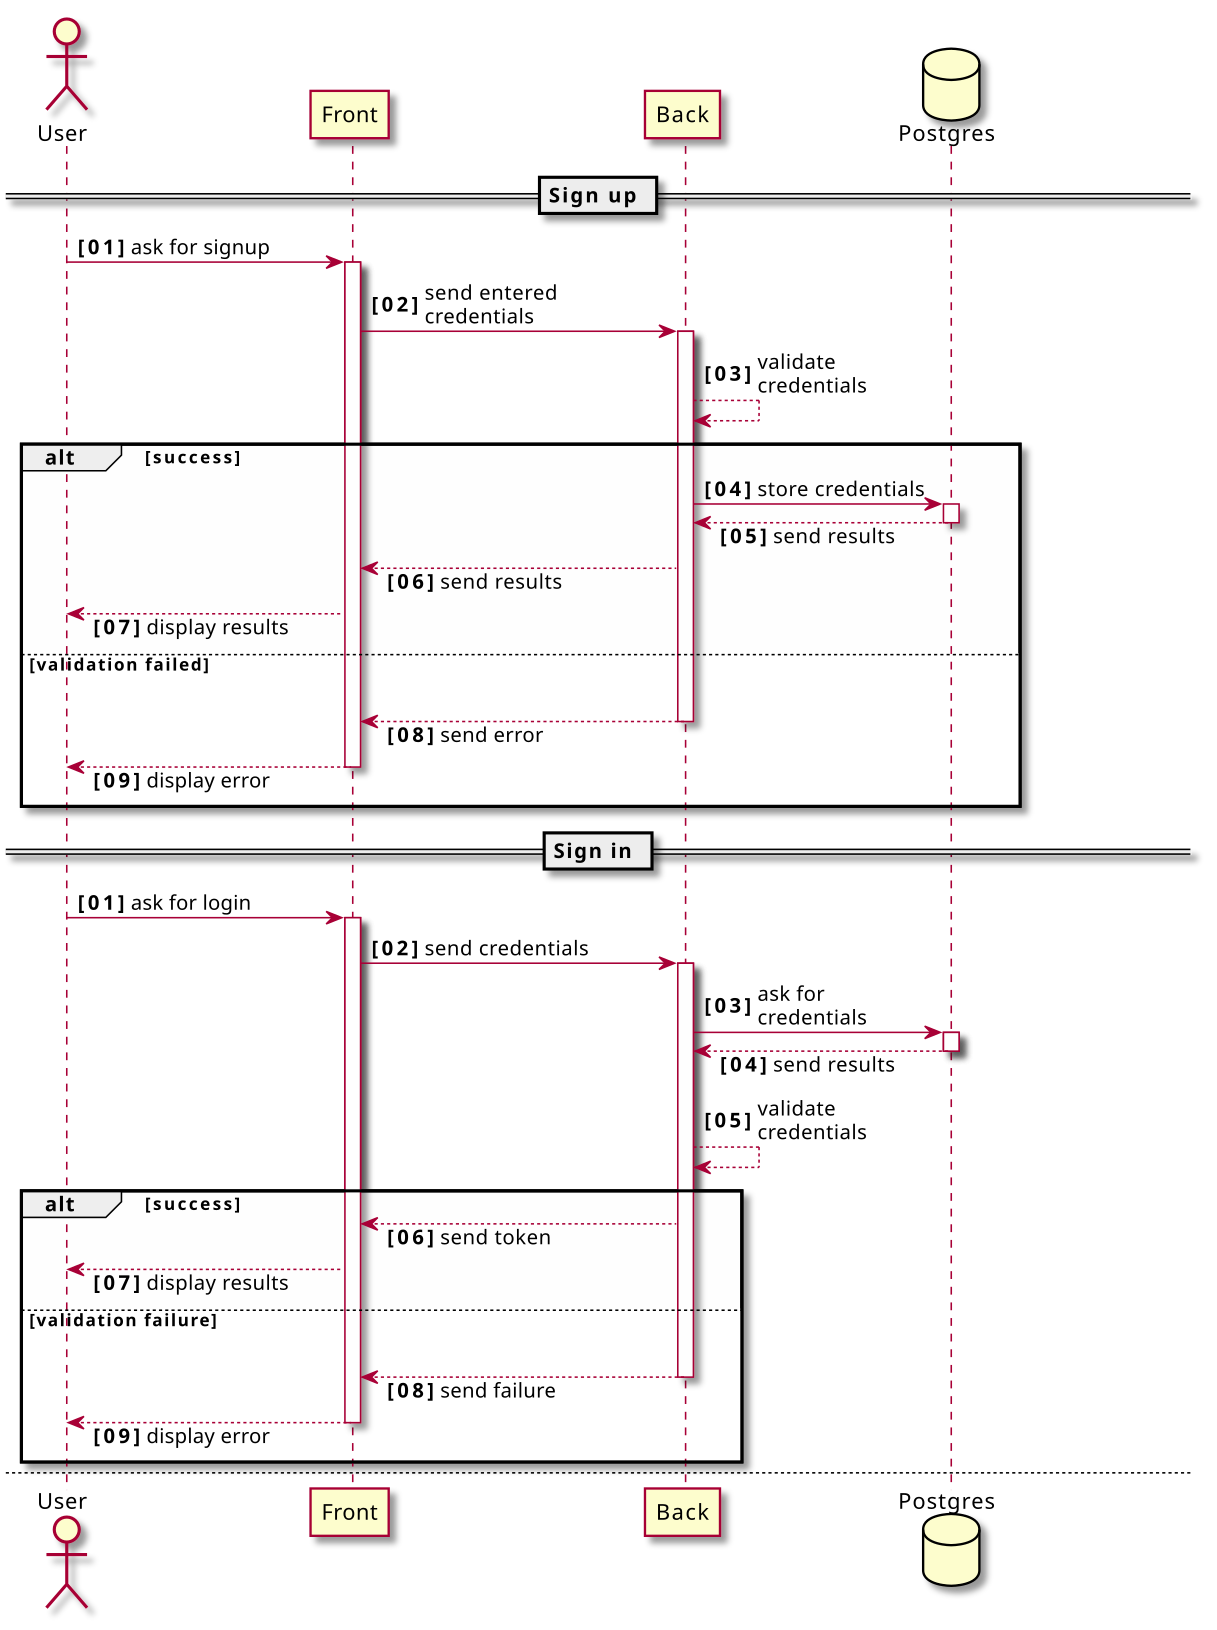
\includegraphics[height=0.7\textheight]{plantuml1.png}
		\caption{Par type de connexion}
	\end{subfigure}
	\caption{Description des flux de données en fonction des cas d'utilisations}
\end{figure}
\begin{figure}[ht]
	\ContinuedFloat\centering
	\begin{subfigure}{\linewidth}
		\centering
		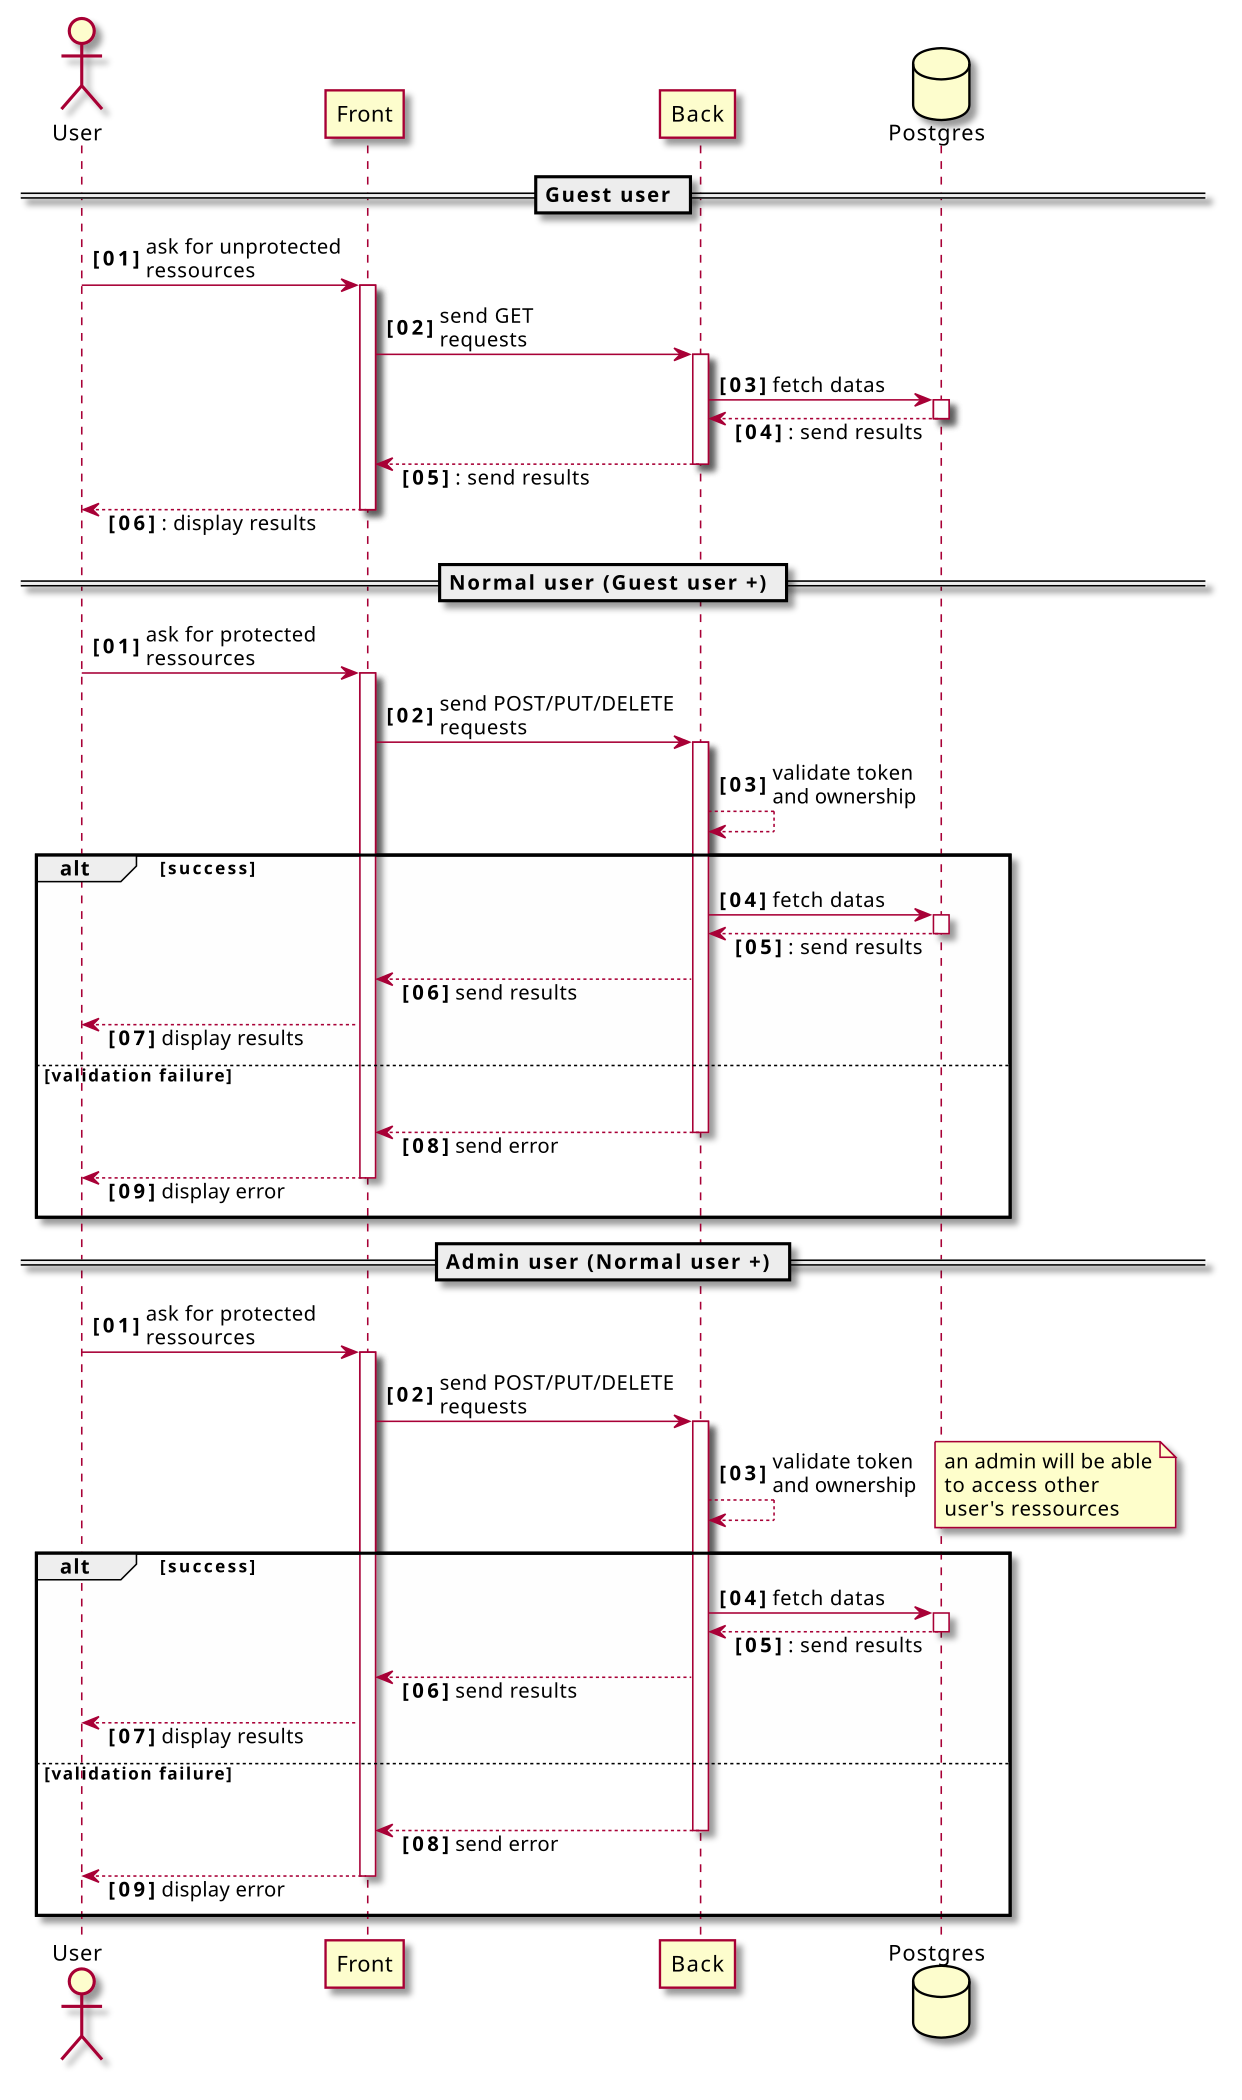
\includegraphics[height=0.75\textheight]{plantuml2.png}
		\caption{Par utilisateur}
	\end{subfigure}
	\caption{Description des flux de données en fonction des cas d'utilisations}
\end{figure}